%==============================================================================
%  MATH 231 -- Linear Algebra I (Queens College, Fall 2026)
%  VECTOR UNIT, PART 4 -- The Standard Basis, Span, and Coordinates
%
%  This is one of the documents covering the vector unit. Section numbering
%  runs CONTINUOUSLY across all parts, so that every cross-reference in the
%  unit means the same thing no matter which part it appears in:
%
%      Part 1  MATH231_vectors_1_definition_and_arithmetic  Sections 1-9
%      Part 2  MATH231_vectors_2_dot_product_and_projection Sections 10-12
%      Part 3  MATH231_vectors_3_norms_and_metrics          Sections 13-15
%      Part 4  MATH231_vectors_4_basis_and_span             Section 16-
%
%  Hence the \setcounter{section}{15} below: this part opens at Section 16.
%  Definitions and examples are numbered BY SECTION so that they too are unique
%  across the whole unit.  References to Sections 1-15 point into Parts 1-3.
%
%  STATUS: in progress.  Further sections will be appended.
%
%  AUDIENCE: distributed to students.  Keep it free of instructor-facing
%  apparatus -- time budgets, pacing notes, teaching cues.
%
%  ONE CORRECTION against the drafted outline, deliberate:
%    the outline wrote  B = { alpha*i + beta*j | alpha, beta in R } = R^2  and
%    called B the basis.  That set is the SPAN of {i, j}, not the basis; the
%    basis is the two-element set {i, j} itself.  This document writes
%    B = {i, j} and span(B) = { alpha*i + beta*j } = R^2, which keeps "i and j
%    span R^2" and "B is a basis for R^2" both literally true.
%
%  NOTATION.  The basis vectors are written with arrows, NOT hats: \hat{u}
%  already means the normalization of u (Sec. 12.1).  Sec. 16.1 does record
%  that these two happen to be unit vectors.
%
%  Compile with pdflatex (standard TeX Live packages only; uses tikz).
%==============================================================================
\documentclass[11pt]{article}

\usepackage[margin=1in]{geometry}
\usepackage{amsmath,amssymb,amsthm}
\usepackage[dvipsnames]{xcolor}
\usepackage{enumitem}
\usepackage{booktabs}
\usepackage{array}
\usepackage[hidelinks]{hyperref}
\usepackage{titlesec}
\usepackage{needspace}
\usepackage{tikz}
\usetikzlibrary{arrows.meta}

%------------------------------------------------------------------ style ----
\titleformat{\section}{\large\bfseries\sffamily}{\thesection.}{0.6em}{}
\titleformat{\subsection}{\normalsize\bfseries\sffamily}{\thesubsection.}{0.5em}{}
\titlespacing*{\section}{0pt}{14pt}{6pt}

\theoremstyle{definition}
\newtheorem{defn}{Definition}[section]
\newtheorem{ex}{Example}[section]
\theoremstyle{remark}
\newtheorem*{rmk}{Remark}
\newtheorem*{warn}{A common confusion}

\newcommand{\lookahead}{\par\smallskip\noindent
  \textbf{\sffamily\textcolor{RoyalBlue}{Looking ahead.}}\ \ignorespaces}

%--------------------------------------------------------------- notation ----
\newcommand{\R}{\mathbb{R}}
\newcommand{\Sph}[1]{\mathbb{S}^{#1}}
\newcommand{\vc}[1]{\mathbf{#1}}
\newcommand{\norm}[1]{\lVert #1\rVert}
\newcommand{\uv}[1]{\hat{\vc{#1}}}
\newcommand{\proj}[2]{\operatorname{proj}_{#1}(#2)}
\newcommand{\comp}[2]{\operatorname{comp}_{#1}(#2)}
\newcommand{\ivec}{\vec{\imath}}
\newcommand{\jvec}{\vec{\jmath}}
\newcommand{\bas}{\mathcal{B}}
\DeclareMathOperator{\spanop}{span}   % \dim is already standard, so not declared

%------------------------------------------------------------- tikz helpers --
\tikzset{
  vecarr/.style   = {-{Stealth[length=2.6mm,width=2.0mm]},very thick},
  thinarr/.style  = {-{Stealth[length=2.2mm,width=1.7mm]},thick},
  axisline/.style = {->,gray!75,thin}
}
% \lattice{xmin}{xmax}{ymin}{ymax}
\newcommand{\lattice}[4]{%
  \draw[step=1cm,gray!25,very thin] (#1,#3) grid (#2,#4);
  \draw[axisline] (#1,0) -- (#2+0.45,0) node[right,font=\scriptsize,black]{$x$};
  \draw[axisline] (0,#3) -- (0,#4+0.45) node[above,font=\scriptsize,black]{$y$};
}

\title{\vspace{-1.2cm}\textbf{\sffamily MATH 231 -- Linear Algebra I}\\[4pt]
       {\large\sffamily The Vector Unit, Part 4 \textbullet\ The Standard
        Basis, Span, and Coordinates}\\[2pt]
       {\normalsize\sffamily Kiely Hall 326 \textbullet\
        Instructor: Kevin Bedoya}}
\author{}
\date{}

\begin{document}
\setcounter{section}{15}  % this part opens at Section 16; see the header note
\maketitle
\vspace{-1.6cm}

\noindent\textbf{About this document.} This is Part 4 of the vector unit.
Section numbering runs continuously through all parts, so a reference such as
\S12.4 points into Part 2 and means exactly what it says:

\begin{center}
\renewcommand{\arraystretch}{1.2}
\begin{tabular}{@{}l l l@{}}
\toprule
\textbf{Part} & \textbf{Sections} & \textbf{Subject} \\
\midrule
1 & \S1--\S9    & vectors, notation, addition, scaling, equality \\
2 & \S10--\S12  & orientation, the dot product, projection \\
3 & \S13--\S15  & Cauchy--Schwarz, metrics, norms \\
4 & \S16--      & the standard basis, span, coordinates \\
\bottomrule
\end{tabular}
\end{center}

\noindent\textbf{Assumed from Parts 1--3.} Addition and scalar multiplication
(\S7--\S8); the bracket notation $\vc{v}=[\,v_1,\,v_2\,]$ and $\R^{2}$ (\S6);
the orthogonality test $\langle\vc{u},\vc{v}\rangle=0$ (\S11.7); the projection
$\proj{\vc{u}}{\vc{v}}$ and component $\comp{\vc{u}}{\vc{v}}$ (\S12.4); and
what it means for two vectors to be parallel (\S10.1).

\medskip
\noindent\textbf{What you should be able to do afterwards.} Write down the
standard basis vectors and verify that they are orthonormal; express any vector
of $\R^{2}$ as a linear combination of them; say what \emph{span} and
\emph{basis} mean; explain what the coordinates of a vector are and why they are
unique; set up the problem of finding coordinates as a linear system; say what
the dimension of a space is and why it agrees with the degrees-of-freedom count
of \S1; produce bases other than the standard one; recognise when two vectors
fail to span the plane; and define linear independence and dependence.

%==============================================================================
\section{The standard basis of \texorpdfstring{$\R^{2}$}{R2}}
%==============================================================================
Since \S6 we have written a vector as a bracketed pair, $\vc{v}=[\,v_1,\,v_2\,]$,
and treated those two numbers as simply given. This section asks where they come
from. The answer is that the bracket notation has been making a silent choice
all along --- and once we see what the choice is, we can start asking what else
could have been chosen.

%------------------------------------------------------------------------------
\subsection{Two special vectors}
%------------------------------------------------------------------------------
\begin{defn}[The standard basis vectors]
The \textbf{standard basis vectors} of $\R^{2}$ are
\[
  \ivec = [\,1,\,0\,],
  \qquad
  \jvec = [\,0,\,1\,] .
\]
They are written with arrows overhead, one of the three conventions of \S6.
\end{defn}

\noindent Geometrically $\ivec$ is one step east and $\jvec$ is one step north:
the two elementary moves, one along each axis.

\begin{center}
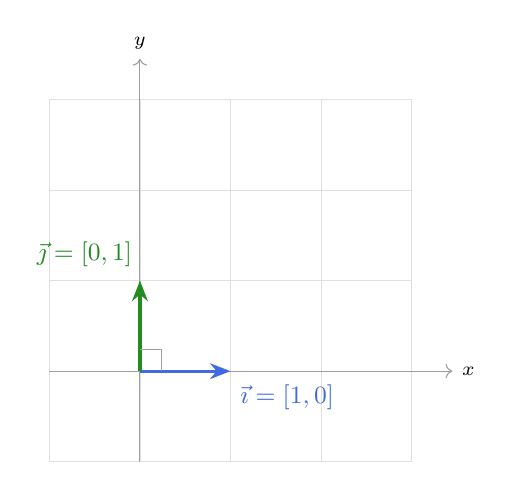
\begin{tikzpicture}[scale=1.15]
  \lattice{-1}{3}{-1}{3}
  \draw[vecarr,RoyalBlue]   (0,0) -- (1,0);
  \draw[vecarr,ForestGreen] (0,0) -- (0,1);
  \draw[gray!75] (0.24,0) -- (0.24,0.24) -- (0,0.24);
  \node[below right,font=\small,RoyalBlue]  at (1.0,-0.04) {$\ivec=[1,0]$};
  \node[above left,font=\small,ForestGreen] at (0.02,1.05) {$\jvec=[0,1]$};
\end{tikzpicture}
\end{center}

\noindent Three properties, each of which we already have the tools to check.

\begin{itemize}[leftmargin=1.4em,itemsep=4pt]
  \item \textbf{Both have unit length.}
        $\norm{\ivec}=\sqrt{1^{2}+0^{2}}=1$ and
        $\norm{\jvec}=\sqrt{0^{2}+1^{2}}=1$, so both lie on the unit circle
        $\Sph{1}$ of \S12.1.
  \item \textbf{They are orthogonal.} Their dot product is
        $\langle\ivec,\jvec\rangle = 1\cdot 0 + 0\cdot 1 = 0$, so by the
        orthogonality test of \S11.7 they meet at a right angle --- as the
        figure shows, since they lie along the two axes.
  \item \textbf{Neither is a multiple of the other.} No scalar $\alpha$
        satisfies $\alpha[1,0]=[0,1]$, since the first coordinate would force
        $\alpha=0$ and the second would force $\alpha\cdot0=1$. So by \S10.1
        they are not parallel. Neither one is redundant: you cannot manufacture
        $\jvec$ out of $\ivec$ alone.
\end{itemize}

\noindent A collection of vectors that are mutually orthogonal and each of unit
length is called \textbf{orthonormal} --- ``ortho'' for the right angles,
``normal'' for the unit lengths. So $\ivec$ and $\jvec$ form an orthonormal
pair, which is as convenient an arrangement as two vectors can have. \S16.4
shows what that convenience buys.

\begin{warn}
This course uses the letters $i$, $j$ and $k$ for three different things, and
you will meet all of them. In the complex numbers lecture, $i$ is the
\emph{imaginary unit} with $i^{2}=-1$, and $i,j,k$ are the \emph{basis elements}
of the quaternions. Here $\ivec$ and $\jvec$ are \emph{vectors} in $\R^{2}$. The
arrows are what tell them apart, so keep them on.
\end{warn}

%------------------------------------------------------------------------------
\subsection{Building vectors out of them}
%------------------------------------------------------------------------------
Take any two real numbers $\alpha$ and $\beta$ and form
\[
  \alpha\ivec + \beta\jvec .
\]
Nothing here is new: it is scalar multiplication from \S8 followed by addition
from \S7. Working it out,
\[
  \alpha\ivec + \beta\jvec
  = \alpha[\,1,\,0\,] + \beta[\,0,\,1\,]
  = [\,\alpha,\,0\,] + [\,0,\,\beta\,]
  = [\,\alpha,\,\beta\,] ,
\]
which is a vector in $\R^{2}$. So every such combination lands inside $\R^{2}$.

\begin{defn}[Linear combination]
An expression of the form $\alpha\vc{u}+\beta\vc{v}$, with $\alpha,\beta\in\R$,
is called a \textbf{linear combination} of $\vc{u}$ and $\vc{v}$.
\end{defn}

\noindent The interesting direction is the reverse one. Does every vector of
$\R^{2}$ arise this way, or do these combinations only reach part of the plane?
They reach all of it, and the proof is a single line: given any
$\vc{v}=[\,v_1,\,v_2\,]$, choose $\alpha=v_1$ and $\beta=v_2$, and
\[
  v_1\ivec + v_2\jvec = [\,v_1,\,v_2\,] = \vc{v} .
\]
Nothing in $\R^{2}$ is missed. Two vectors, scaled and added, generate the
entire plane --- which is why $\ivec$ and $\jvec$ deserve to be called the
\emph{scaffolding} of $\R^{2}$: build them once and everything else follows.

%------------------------------------------------------------------------------
\subsection{Span and basis}
%------------------------------------------------------------------------------
Those two paragraphs proved two inclusions, and together they deserve a name.

\begin{defn}[Span]
The \textbf{span} of a collection of vectors is the set of \emph{all} their
linear combinations. For $\ivec$ and $\jvec$,
\[
  \spanop\{\ivec,\jvec\}
  \;=\;
  \bigl\{\, \alpha\ivec + \beta\jvec \;\bigm|\; \alpha,\beta\in\R \,\bigr\}.
\]
\end{defn}

\noindent The first calculation of \S16.2 showed
$\spanop\{\ivec,\jvec\}\subseteq\R^{2}$, and the second showed
$\R^{2}\subseteq\spanop\{\ivec,\jvec\}$. Both inclusions hold, so
\[
  \boxed{\;\spanop\{\ivec,\jvec\} \;=\; \R^{2}\;}
\]
and we say that $\ivec$ and $\jvec$ \textbf{span} $\R^{2}$.

\begin{defn}[Basis, working definition]
A collection of vectors is a \textbf{basis} for a space when it spans that space
and does so without redundancy --- no vector in the collection is a linear
combination of the others, so none of them can be dropped. We write
\[
  \bas = \{\,\ivec,\ \jvec\,\} ,
\]
and call $\bas$ the \textbf{standard basis} of $\R^{2}$.
\end{defn}

\begin{rmk}[Basis and span are different objects]
Keep the two apart. The basis $\bas=\{\ivec,\jvec\}$ is a set containing
\emph{two vectors}. Its span, $\spanop\bas=\R^{2}$, is a set containing
\emph{infinitely many} --- every vector in the plane. A basis is small; what it
generates is large. That is the entire point of a basis: it is a finite
description of an infinite set.
\end{rmk}

\noindent Redundancy is the clause worth dwelling on. Spanning alone is easy to
achieve by piling on extra vectors: the collection
$\{\ivec,\jvec,[\,3,\,5\,]\}$ also spans $\R^{2}$, but the third vector earns
nothing, since $[\,3,\,5\,]=3\ivec+5\jvec$ was already reachable. A basis is
required to carry no such passengers, and \S16.1 checked that ours does not:
neither $\ivec$ nor $\jvec$ is a multiple of the other.

\lookahead ``Without redundancy'' is doing real work here and deserves a
sharper statement than the one above. It has a proper name --- \emph{linear
independence} --- and a definition that applies to any number of vectors at
once, not just two. We will meet it shortly.

%------------------------------------------------------------------------------
\subsection{Coordinates}
%------------------------------------------------------------------------------
\begin{defn}[Coordinates]
If $\vc{v}=\alpha\ivec+\beta\jvec$, the scalars $\alpha$ and $\beta$ are the
\textbf{coordinates} of $\vc{v}$ with respect to the basis $\bas$.
\end{defn}

\noindent For the word ``the'' to be justified, there had better be only one
such pair --- and there is. Suppose a vector could be written two ways,
\[
  \alpha\ivec + \beta\jvec = \alpha'\ivec + \beta'\jvec .
\]
Both sides evaluate componentwise to $[\,\alpha,\,\beta\,]$ and
$[\,\alpha',\,\beta'\,]$, and two vectors are equal exactly when their
coordinates agree (\S9). So $\alpha=\alpha'$ and $\beta=\beta'$: the two
representations were the same one. Coordinates are \textbf{unique}.

\begin{rmk}[What the bracket notation was hiding]
Look again at $\vc{v}=[\,v_1,\,v_2\,]$. We have just shown
$\vc{v}=v_1\ivec+v_2\jvec$, so the two numbers inside the brackets are exactly
the coordinates of $\vc{v}$ with respect to $\bas$. The notation of \S6 was
never neutral --- it silently reported coordinates in one particular basis. We
have been able to ignore this only because $\bas$ has been the sole basis in
play. Other bases exist, and the same vector has different coordinates in each.
\end{rmk}

\begin{rmk}[Why reading them off is free]
There is a reason the coordinates turned out to be the components themselves.
Because $\bas$ is orthonormal, the projection machinery of \S12.4 collapses:
\[
  \comp{\ivec}{\vc{v}}
  = \frac{\langle\ivec,\vc{v}\rangle}{\norm{\ivec}}
  = \frac{1\cdot v_1 + 0\cdot v_2}{1}
  = v_1 ,
\]
and likewise $\comp{\jvec}{\vc{v}}=v_2$. So the coordinate of $\vc{v}$ along a
basis vector \emph{is} its projection component onto that basis vector --- the
shadow it casts on each axis. Orthonormality is what makes the norms $1$ and the
cross terms $0$, and so makes the arithmetic vanish.
\end{rmk}

%------------------------------------------------------------------------------
\subsection{The reverse problem, and a first linear system}
%------------------------------------------------------------------------------
Turn the question around. Instead of being handed $\alpha$ and $\beta$ and
asked what they build, start with a vector $\vc{v}\in\R^{2}$ and treat the
scalars as \emph{unknowns}:
\[
  \vc{v} = \alpha\ivec + \beta\jvec ,
  \qquad \alpha,\beta \text{ to be found.}
\]
Two facts already settle that this is a sensible question. Because $\ivec$ and
$\jvec$ span $\R^{2}$, a solution \emph{exists} --- no vector of the plane is
out of reach. Because coordinates are unique, the solution is the \emph{only}
one. We are not searching hopefully; we are computing something we know is there
and know is unambiguous.

\subsubsection*{The picture}
Geometrically the answer is a walk. Starting at the origin, travel $\alpha$
steps along $\ivec$ --- purely horizontal --- and then, from where you land,
$\beta$ steps along $\jvec$ --- purely vertical. That is the head-to-tail
reading of addition from \S7.1, and the question is how far to walk in each
direction to arrive exactly at the head of $\vc{v}$.

Read the other way, the dashed guides drop from the head of $\vc{v}$ onto the
two axes, and where they land is the answer.

\begin{center}
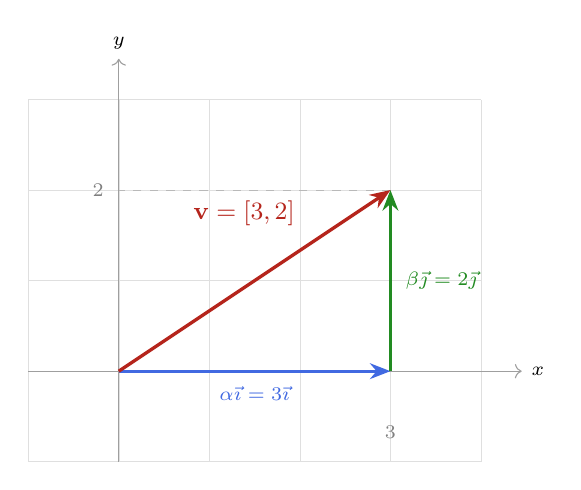
\begin{tikzpicture}[scale=1.15]
  \lattice{-1}{4}{-1}{3}
  \draw[gray!55,dashed] (3,2) -- (3,0);
  \draw[gray!55,dashed] (3,2) -- (0,2);
  \draw[vecarr,RoyalBlue]   (0,0) -- (3,0);
  \draw[vecarr,ForestGreen] (3,0) -- (3,2);
  \draw[vecarr,BrickRed]    (0,0) -- (3,2);
  \node[below,font=\scriptsize,RoyalBlue]      at (1.5,-0.06) {$\alpha\ivec=3\ivec$};
  \node[right,font=\scriptsize,ForestGreen]    at (3.06,1.0)  {$\beta\jvec=2\jvec$};
  \node[above left,font=\small,BrickRed]       at (2.05,1.5)  {$\vc{v}=[3,2]$};
  \node[left,font=\scriptsize,gray]            at (-0.06,2)   {$2$};
  \node[below,font=\scriptsize,gray]           at (3,-0.5)    {$3$};
\end{tikzpicture}
\end{center}

\subsubsection*{Writing it as a system}
Now do it algebraically. Expand the right-hand side componentwise:
\[
  \alpha\ivec + \beta\jvec
  = [\,\alpha\cdot 1 + \beta\cdot 0,\;\; \alpha\cdot 0 + \beta\cdot 1\,] .
\]
Setting this equal to $\vc{v}=[\,v_1,\,v_2\,]$ and matching coordinates gives
two equations in the two unknowns:
\[
  \begin{aligned}
    v_1 &= \alpha\cdot 1 + \beta\cdot 0, \\
    v_2 &= \alpha\cdot 0 + \beta\cdot 1 .
  \end{aligned}
\]
A collection of equations like this --- several linear equations sharing the
same unknowns, to be satisfied simultaneously --- is called a \textbf{linear
system}. This one barely deserves the name, because the zeros knock out one term
in each equation and it collapses on sight:
\[
  v_1 = \alpha,
  \qquad
  v_2 = \beta .
\]

\begin{ex}
For $\vc{v}=[\,3,\,2\,]$ the system gives $\alpha=3$ and $\beta=2$, so
$\vc{v}=3\ivec+2\jvec$ --- the walk in the figure above. For
$\vc{v}=[\,-2,\,5\,]$ it gives $\vc{v}=-2\ivec+5\jvec$: two steps west, then
five north.
\end{ex}

\begin{rmk}
Do not mistake how easy that was for how easy the question is. The system
collapsed because the coefficient of $\beta$ in the first equation and of
$\alpha$ in the second were both $0$, and those zeros are precisely the
statement $\langle\ivec,\jvec\rangle=0$ --- the orthogonality we checked in
\S16.1, reappearing as the arithmetic that makes the work disappear. The
standard basis is engineered so that reading coordinates costs nothing.
\end{rmk}

\lookahead Ask the same question against a basis that is \emph{not} the standard
one and the zeros are gone. The two equations then genuinely interact, both
unknowns appear in both, and the system must actually be solved. That is the
general problem of linear systems --- how to state it, when it has a solution,
how many solutions there can be, and how to compute them --- and it will occupy
a substantial part of this course. The trivial case above is worth remembering
as the one you are always trying to get back to.

%==============================================================================
\section{Dimension}
%==============================================================================
A basis carries a number with it, and that number turns out to be one we have
been using informally since \S1.

\begin{defn}[Dimension]
The \textbf{dimension} of a space is the number of vectors in a basis for it.
\end{defn}

\noindent Our basis $\bas=\{\ivec,\jvec\}$ contains two vectors, so
\[
  \dim\R^{2} = 2 .
\]
The superscript in $\R^{2}$ was telling us the dimension all along.

\subsection*{Why this agrees with what we already meant}
In \S1 we described dimension as a \emph{degree of freedom} with respect to
spatial coordinates: how many independent numbers must you supply to pin down a
position? The two accounts are the same account. Supplying a position in
$\R^{2}$ means supplying its two coordinates $\alpha$ and $\beta$ --- one per
basis vector --- so the count of free numbers and the count of basis vectors are
forced to agree.

Read geometrically, the dimension counts \textbf{independent directions}. The
basis $\bas$ offers two: along the $x$-axis and along the $y$-axis. Neither can
be obtained from the other, and once both are available, nothing further is
needed.

\begin{warn}
``Two independent directions'' does not mean the basis represents only two
directions. It represents \emph{every} direction in the plane --- the vector
$3\ivec+2\jvec$ points in a direction that is neither of the two axes. What the
number $2$ counts is how many directions you must be \emph{given} before all the
rest come free. Two is the number of directions that are independent, not the
number that are reachable.
\end{warn}

%==============================================================================
\section{Other bases, and linear independence}
%==============================================================================
Nothing in \S16.3 said the standard basis is the \emph{only} basis for $\R^{2}$.
It is merely the most convenient one. Once we go looking for others, a question
appears that the standard basis was too well behaved to raise: which pairs of
vectors work, and which fail?

%------------------------------------------------------------------------------
\subsection{Bases other than the standard one}
%------------------------------------------------------------------------------
Consider the pairs
\[
  \vc{u}=[\,1,\,2\,],\ \vc{v}=[\,2,\,3\,]
  \qquad\text{and}\qquad
  \vc{u}=[\,2,\,3\,],\ \vc{v}=[\,3,\,4\,] .
\]
Neither pair looks anything like $\{\ivec,\jvec\}$ --- the vectors are not unit
length, not orthogonal, not aligned with the axes --- and yet each pair is a
perfectly good basis for $\R^{2}$.

\begin{center}
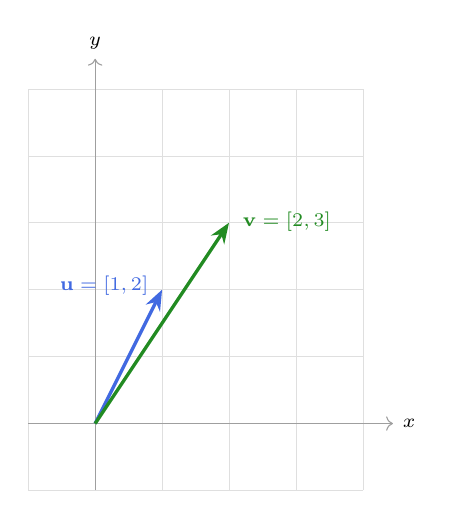
\begin{tikzpicture}[scale=0.85,baseline=(current bounding box.center)]
  \lattice{-1}{4}{-1}{5}
  \draw[vecarr,RoyalBlue]   (0,0) -- (1,2);
  \draw[vecarr,ForestGreen] (0,0) -- (2,3);
  \node[left,font=\scriptsize,RoyalBlue]    at (0.94,2.06) {$\vc{u}=[1,2]$};
  \node[right,font=\scriptsize,ForestGreen] at (2.06,3.02) {$\vc{v}=[2,3]$};
\end{tikzpicture}
\hspace{1.1cm}
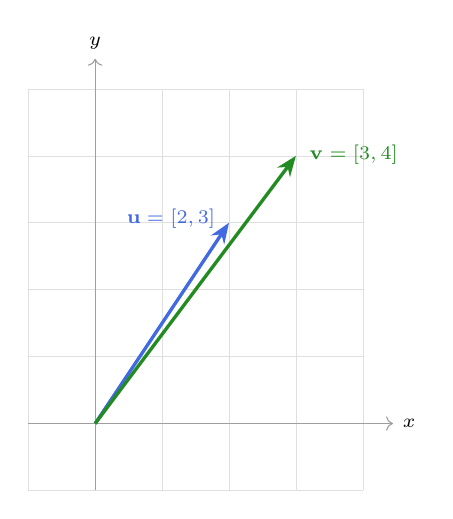
\begin{tikzpicture}[scale=0.85,baseline=(current bounding box.center)]
  \lattice{-1}{4}{-1}{5}
  \draw[vecarr,RoyalBlue]   (0,0) -- (2,3);
  \draw[vecarr,ForestGreen] (0,0) -- (3,4);
  \node[left,font=\scriptsize,RoyalBlue]    at (1.94,3.06) {$\vc{u}=[2,3]$};
  \node[right,font=\scriptsize,ForestGreen] at (3.06,4.02) {$\vc{v}=[3,4]$};
\end{tikzpicture}
\end{center}

\noindent Being a basis costs something, though: the coordinates are no longer
free to read off.

\begin{ex}[Coordinates against a non-standard basis]
Take the basis $\{\vc{u},\vc{v}\}$ with $\vc{u}=[1,2]$ and $\vc{v}=[2,3]$, and
ask for the coordinates of $\vc{w}=[\,1,\,0\,]$. We need $\alpha,\beta$ with
$\alpha\vc{u}+\beta\vc{v}=\vc{w}$, which componentwise is
\[
  \begin{aligned}
    \alpha\cdot 1 + \beta\cdot 2 &= 1, \\
    \alpha\cdot 2 + \beta\cdot 3 &= 0 .
  \end{aligned}
\]
No zeros this time, so nothing collapses. The second equation gives
$\alpha=-\tfrac32\beta$; substituting into the first,
$-\tfrac32\beta+2\beta=\tfrac12\beta=1$, so $\beta=2$ and $\alpha=-3$. Checking:
\[
  -3[\,1,\,2\,] + 2[\,2,\,3\,] = [\,-3,\,-6\,]+[\,4,\,6\,] = [\,1,\,0\,] .
  \quad\checkmark
\]
So $\vc{w}$ has coordinates $-3$ and $2$ in this basis, where in the standard
basis it had coordinates $1$ and $0$. Same vector, different numbers --- exactly
what the remark in \S16.4 warned. And this is the situation \S16.5 pointed at:
away from the standard basis, finding coordinates is a genuine linear system
that has to be solved.
\end{ex}

%------------------------------------------------------------------------------
\subsection{When two vectors do not span the plane}
%------------------------------------------------------------------------------
Now try
\[
  \vc{u}=[\,1,\,2\,],
  \qquad
  \vc{v}=[\,2,\,4\,] .
\]
Plot them and something is visibly wrong: both arrows lie along one and the same
line through the origin.

\begin{center}
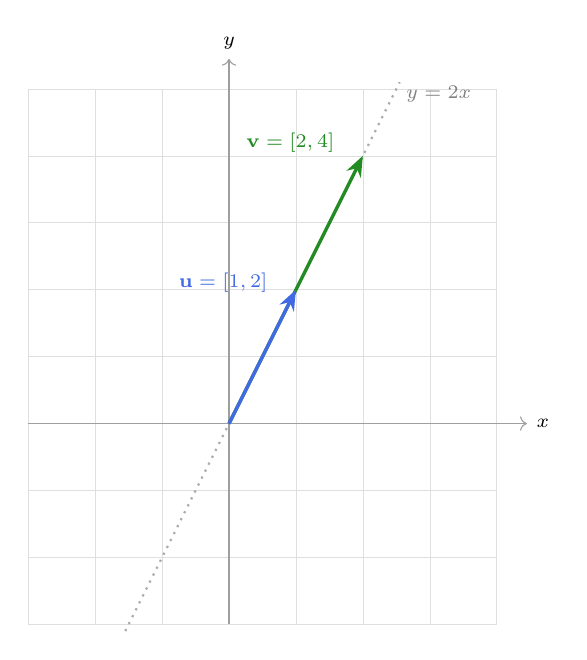
\begin{tikzpicture}[scale=0.85]
  \lattice{-3}{4}{-3}{5}
  % the line spanned by u -- every combination of u and v lands on it
  \draw[gray!65,dotted,thick] (-1.55,-3.1) -- (2.55,5.1);
  \draw[vecarr,ForestGreen] (0,0) -- (2,4);
  \draw[vecarr,RoyalBlue]   (0,0) -- (1,2);
  % keep the labels clear of the line the two vectors sit on
  \node[left,font=\scriptsize,RoyalBlue]   at (0.72,2.10) {$\vc{u}=[1,2]$};
  \node[left,font=\scriptsize,ForestGreen] at (1.72,4.20) {$\vc{v}=[2,4]$};
  \node[right,font=\scriptsize,gray]       at (2.5,4.92)  {$y=2x$};
\end{tikzpicture}
\end{center}

\noindent The reason is immediate: $\vc{v}=2\vc{u}$. And that single fact
collapses every linear combination onto the same line:
\[
  \alpha\vc{u} + \beta\vc{v}
  = \alpha\vc{u} + \beta(2\vc{u})
  = (\alpha+2\beta)\,\vc{u} ,
\]
which is a scalar multiple of $\vc{u}$ --- and by \S8 every scalar multiple of
$\vc{u}$ lies on the line through the origin and the head of $\vc{u}$. Whatever
$\alpha$ and $\beta$ you choose, you never leave that line.

So there is no way to assign coordinates to a point off the line: the point is
simply not reachable. These two vectors span only a \emph{subset} of the plane,
and therefore
\[
  \spanop\{\vc{u},\vc{v}\} \neq \R^{2}
  \qquad\text{when}\qquad
  \vc{u}=[1,2],\ \vc{v}=[2,4].
\]
Two vectors are not automatically a basis for $\R^{2}$. Having the right
\emph{number} of vectors is not enough; they have to stand in the right
relationship to one another.

%------------------------------------------------------------------------------
\subsection{Three questions}
%------------------------------------------------------------------------------
That failure is worth more than the successes, because it tells us there is
something to characterise. Three questions follow, and we take them one at a
time.

\begin{enumerate}[label=\textbf{Q\arabic*.},leftmargin=3.0em,itemsep=5pt,
                  topsep=5pt]
  \item Which pairs of vectors form a basis for $\R^{2}$ --- that is, which
        pairs span $\R^{2}$?
  \item The pair $[\,1,\,2\,]$ and $[\,2,\,4\,]$ failed to span $\R^{2}$, but
        they clearly span \emph{something}. What kind of basis do they form?
  \item How many different bases does $\R^{2}$ have?
\end{enumerate}

%------------------------------------------------------------------------------
\subsection{Question 1: linear independence}
%------------------------------------------------------------------------------
Q1 is better asked as a question about a \emph{relationship}: what must be true
of two vectors, with respect to each other, for them to form a basis?

The two examples answer it geometrically. The vectors $[2,3]$ and $[3,4]$ point
in genuinely different directions, and no amount of stretching turns one into
the other: there is no scalar $\alpha$ with $\alpha[2,3]=[3,4]$, since the first
coordinate demands $\alpha=\tfrac32$ and the second then gives
$\tfrac32\cdot3=\tfrac92\neq4$. The pair $[1,2]$ and $[2,4]$ fails exactly here:
$2\cdot[1,2]=[2,4]$, so one \emph{is} a stretch of the other, and that is what
flattened their span onto a line.

So the property we want is ``neither vector is a scalar multiple of the other''
--- which is the \emph{not parallel} of \S10.1. That phrasing is correct, but it
is awkward: it treats the two vectors asymmetrically, and it does not generalise
past two. The standard formulation fixes both problems by asking instead about
combinations that produce the zero vector:
\[
  \alpha[\,2,\,3\,] + \beta[\,3,\,4\,] = \vc{0}
  \qquad\Longleftrightarrow\qquad
  \alpha=\beta=0 .
\]
Read the left-to-right direction as the real content: the \emph{only} way to
combine these two vectors and land back at the origin is to take nothing of
either.

\begin{defn}[Linear independence and dependence in $\R^{2}$]
Two vectors $\vc{u},\vc{v}\in\R^{2}$ are \textbf{linearly independent} when the
only scalars $\alpha,\beta\in\R$ satisfying
\[
  \alpha\vc{u} + \beta\vc{v} = \vc{0}
\]
are $\alpha=0$ and $\beta=0$.

They are \textbf{linearly dependent} when they are not --- that is, when there
exist scalars $\alpha,\beta$, \emph{not both zero}, with
$\alpha\vc{u}+\beta\vc{v}=\vc{0}$.
\end{defn}

\begin{rmk}[Why ``not both zero'' cannot be dropped]
The choice $\alpha=\beta=0$ always works, for any two vectors whatsoever, since
$0\vc{u}+0\vc{v}=\vc{0}$ is automatic. It carries no information. So a
definition of dependence reading ``there exist $\alpha,\beta$ with
$\alpha\vc{u}+\beta\vc{v}=\vc{0}$'' would be satisfied by every pair and would
say nothing at all. The clause \emph{not both zero} is what gives the definition
teeth --- and for the same reason, independence is stated as
$\alpha=\beta=0$ being the \emph{only} solution.
\end{rmk}

\begin{ex}[The two pairs, checked]
For $\vc{u}=[1,2]$ and $\vc{v}=[2,4]$, take $\alpha=2$ and $\beta=-1$:
\[
  2[\,1,\,2\,] + (-1)[\,2,\,4\,] = [\,2,\,4\,] - [\,2,\,4\,] = \vc{0} ,
\]
and those scalars are not both zero. So the pair is linearly
\textbf{dependent} --- and we have already seen the consequence: their span is a
line, not the plane.

For $\vc{u}=[2,3]$ and $\vc{v}=[3,4]$, suppose
$\alpha[2,3]+\beta[3,4]=\vc{0}$. Componentwise that is $2\alpha+3\beta=0$ and
$3\alpha+4\beta=0$. The first gives $\alpha=-\tfrac32\beta$; substituting into
the second, $-\tfrac92\beta+4\beta=-\tfrac12\beta=0$, so $\beta=0$ and then
$\alpha=0$. The only solution is the trivial one, so the pair is linearly
\textbf{independent}.
\end{ex}

\begin{rmk}[For two vectors, dependence is exactly parallelism]
When $\vc{u}$ and $\vc{v}$ are both nonzero, linear dependence says nothing more
than what \S10.1 called parallel. If $\alpha\vc{u}+\beta\vc{v}=\vc{0}$ with, say,
$\alpha\neq0$, then $\vc{u}=-\tfrac{\beta}{\alpha}\vc{v}$, so each is a scalar
multiple of the other; and conversely a multiple relation rearranges into such a
combination. The one wrinkle is the zero vector: $\{\vc{0},\vc{v}\}$ is always
dependent, since $1\cdot\vc{0}+0\cdot\vc{v}=\vc{0}$ uses a nonzero scalar --- yet
\S10.1 deliberately excluded $\vc{0}$ from the word ``parallel'' because it has
no direction. The combination formulation handles that case without special
pleading, which is one more reason it is the definition of record.
\end{rmk}

\noindent This answers Q1, at least for pairs: \textbf{two vectors form a basis
for $\R^{2}$ precisely when they are linearly independent.} Independence is what
guarantees the two arrows genuinely open the plane out, instead of collapsing it
onto a line.

\lookahead The definition above was written for two vectors so that it can be
checked by hand, but nothing in it depends on there being two. The general
version asks the same question of any collection --- when is the zero vector
reachable only by taking nothing of everything? --- and that is the version we
will need once we leave the plane. Q2 and Q3 remain open.

\end{document}
